\chapter{Diseño}
\label{sec:diseno}

%Es uno de los capítulos más importantes. Debe explicar claramente la solución propuesta justificando la aproximación adoptada. Este capítulo, según el caso, es aconsejable que defina claramente la arquitectura del sistema propuesto, identificando los roles o partes o actores del sistema. Pueden emplearse metodologías basadas en diagramas de clases, paquetes, diagramas secuenciales, diagramas de relación, etc.

%Si se ha diseñado una interfaz gráfica debe también describirse su estructura, dónde se mostrará la información, etc.


La figura \ref{fig:diag-bloques} muestra un diagrama con los bloques con el diseño general del proyecto. En el docker se incluye el \textit{deployer} que instala el \textit{core} de la cadena de bloques. Además, se encuentra la base de datos \texttt{postgresql}, que estará en interacción con el \textit{core} para almacenar la información en la misma.\\

Por otra parte, fuera del docker, se encuentra el \textit{explorer} y la aplicación Desktop Wallet. El \textit{explorer} estará conectado al \textit{core} mediante el puerto API $4102$, al \textit{explorer} se podrá acceder mediante un navegador con la dirección\mbox{\texttt{http://NODE\_GENESIS:4200}}. Sin embargo, para acceder a la aplicación Desktop Wallet será necesario descargarla, veáse apéndice manual de usuario \ref{sec:manual-wallet}, dicha apliación se conectará con el \textit{core} mediante el puerto API $4103$.

%Los nombres de la bases de datos se pueden ver con el comando psql -l, y podemos ver que hay una para cada red, a nosotros no interesa core_bridgechain_testnet. Para visualizar las tablas poner el comando psql -U deployer - d core_bridgechain_testnet.

\begin{figure}[H]
	\centering
	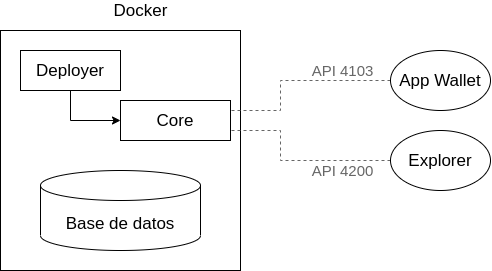
\includegraphics[width=0.8\textwidth]{figuras/diagrama_bloquesARK.png}
	\caption{Diagrama de bloques}
	\label{fig:diag-bloques}
\end{figure}


\section{Algoritmo criptográfico}

La estructura del algoritmo viene dada por un fichero escrito en python donde se encuentran las funciones que se explicarán en detalle en el capítulo \ref{sec:implementacion}.

El fichero \texttt{uov.py} incorpora main con un ejemplo de uso del algoritmo independientemente de la \textit{blockchain}.

\section{Ecosistema ARK}

El ecosistema ark se ha instalado en un docker \texttt{ubuntu:xenial}. En el \textit{home} del mismo, nos encontramos con las tres carpetas necesarias para la ejecución e instalación tanto de la \textit{blockchain} y como del \textit{explorer}, estas son \texttt{deployer}, \texttt{core-bridgechain} y \texttt{core-explorer}. A continuación se van a explicar para que sirven las dos primeras, puesto que del \texttt{core-explorer} no ha habido ninguna modificación y se ha usado con todos los valores por defecto.\\



\subsection{Directorio deployer}
La carpeta \texttt{deployer} contiene varios directorios y ficheros siendo los más importantes, \texttt{app}, \texttt{bridgechain.sh}, \texttt{setup.sh}, ver árbol de directorio \ref{tree:depl}.


\begin{figure}[H]
	\begin{forest}
	  for tree={
		font=\scriptsize\sffamily,
		grow'=0,
		child anchor=west,
		parent anchor=south,
		anchor=west,
		calign=first,
		inner xsep=7pt,
		edge path={
		  \noexpand\path [draw, \forestoption{edge}]
		  (!u.south west) +(5pt,0) |- (.child anchor) pic {folder} \forestoption{edge label};
		},
		file/.style={edge path={\noexpand\path [draw, \forestoption{edge}]
		      (!u.south west) +(5pt,0) |- (.child anchor) \forestoption{edge label};},
		      inner xsep=2pt,font=\tiny\sffamily
		},
		before typesetting nodes={
		  if n=1
		    {insert before={[,phantom]}}
		    {}
		},
		fit=band,
		before computing xy={l=15pt},
	  } 
		[deployer
		  [app
			[app-core.sh, file]
			[app-explorer.sh, file]
		  ]
		  [bridgechain.sh, file]
		  [setup.sh, file]
		]
	\end{forest}
	\caption{Árbol de directorios de deployer}
	\label{tree:depl}
\end{figure}

\begin{itemize}
	\item El directorio \texttt{app} contiene a su vez dos ficheros, \texttt{app-core.sh} que clona e instala el repositorio de github \texttt{mvictoria1997/core} puesto que se ha cambiado la línea 108 para tal fin, código \ref{cod:app-core}, en su defecto instalaría la \textit{blockchain} de \mbox{ArkEcosystem}. Este cambio se hace para obtener en la \textit{blockchain} las modificaciones en el algoritmo de firma.

	\begin{lstlisting}[language=Python,caption=Línea 108 app-core.sh, label=cod:app-core]
		git clone https://github.com/mvictoria1997/core.git --single-branch "$BRIDGECHAIN_PATH"
	\end{lstlisting}

	El segundo archivo, \texttt{app-explorer.sh},  clona e instala el repositorio de github \texttt{ArkEcosystem/explorer} no se hace ningún cambio puesto que se va a utilizar todo por defecto.

	\item El archivo \texttt{bridgchain.sh} ejecuta los archivos \texttt{app-core.sh} y \texttt{app-explorer.sh} para instalar la \textit{blockchain} y el \textit{explorer} respectivamente.
	\item El archivo \texttt{setup.sh} realiza una instalación inicial del repositorio.
\end{itemize}


\subsection{Directorio core-bridgechain}

El directorio \texttt{core-bridgechain} contiene cinco directorios importantes, \texttt{blocks}, \texttt{crypto}, \texttt{identities}, \texttt{interfaces} y \texttt{transactions}, ver árbol de directorios \ref{tree:core-b}.

\begin{itemize}
	\item Directorio \texttt{blocks} gestiona los bloques de la \textit{blockchain}, en este directorio se encuentran los ficheros, \texttt{block.ts} que engloba las funciones de verificación de la firma de los bloques y \texttt{factory.ts} que administra la creación y firma de los bloques.
	\item En el directorio \texttt{crypto} es donde se han realizado los cambios, puesto que se encuentran los ficheros con los algoritmos de firma y verificación (objetivo de nuestro proyecto). Podemos distinguir tres tipos de ficheros, los escritos en \texttt{typescript}, los escritos en \texttt{python} y por último los de almacenamiento con extensión \texttt{json}.
	
	De los escritos en \texttt{typescript} destaca el fichero \texttt{hash.ts}, en él se encuentran las funciones de firma y verificación de tres algoritmos, \acrshort{ecdsa}, Schnorr\cite{schnorr} y \acrshort{uov} (la añadida para este trabajo). Para no tener que modificar las funciones desde donde se realizan las llamadas a los distintos algoritmos, lo que se ha hecho es llamar desde la función de firma y verificación del algoritmo ECDSA a las funciones de firma y verificación del algoritmo UOV, respectivamente.
	
	En los archivos de \texttt{python} se encuentran \texttt{uov.py}, \texttt{signature.py} y \texttt{verify.py}. El archivo \texttt{uov.py} contiene las funciones del algoritmo UOV, estas se explicarán en el capítulo \ref{sec:implementacion}. Los otros dos archivos son de transición, esto es, se llaman desde la función de firma a \texttt{signature.py} y desde la función de verificación a \texttt{verify.py}, para pasar los parámetros del lenguaje \texttt{typescript} al lenguaje \texttt{python}, a continuación se realizan llamadas a las funciones de firma o verificación, volviendo a pasar los resultados a las funciones de \texttt{typescript}.
	
	Por último han de destacarse los ficheros de almacenamiento \texttt{data.json} y \texttt{signature.json}. En \texttt{data.json} podemos encontrar cada una de las claves públicas y privadas generadas para el algoritmo de Schnorr y las correspondientes para el algoritmo UOV (los $\alpha$ y $\beta$ privados y públicos), cada conjunto de claves se ha almacenado en un diccionario con la estructura que muestra el código \ref{cod:data-json}. Debido a los problemas explicados en el apartado de análisis \ref{sec:analisis-analisis}, el archivo \texttt{signature.json} contiene las firmas en hexadecimal y sus correspondientes en forma de vector, tal y como muestra el código \ref{cod:sign-json}.
	
	\begin{lstlisting}[language=Python,caption=Estructura archivo data.json, label=cod:data-json]
		{
			"id":
			"pub_schnorr":
			"priv_schnorr":
			"priv_alpha_UOV": 
			"priv_beta_OUV": 
			"pub_alpha_UOV": 
			"pub_beta_OUV": 
		}
	\end{lstlisting}
	
	\begin{lstlisting}[language=Python,caption=Estructura archivo signature.json, label=cod:sign-json]
		{
			"hex":
			"vector":
		}
	\end{lstlisting}
	
	\item Directorio \texttt{identities} abarca la creación y almacenamiento de las claves pública y privada.
	\item Directorio \texttt{interfaces} incluye las interfaces, esto es, los campos que se requieren para la creación de cada objeto o los que pueden añadirse posteriormente. Los objetos más destacados y con los que se han trabajado son bloques, identidades, mensajes y transacciones.
	
	Los bloques se muestran en el archivo \texttt{blocks.ts}, las identidades (con las claves pública y privada) en el archivo \texttt{identities.ts}, los mensajes en el archvio \texttt{message.ts}, y las transacciones en el archivo \texttt{transactions.ts}.
	\item Entre los ficheros del directorio \texttt{transactions} podemos encontrar \texttt{signer.ts} y \texttt{verifier.ts}. El primero contiene la gestión de la firma de transacciones y el segundo la verificación de la firma.
\end{itemize}

\begin{figure}[H]
	\begin{forest}
	  for tree={
		font=\scriptsize\sffamily,
		grow'=0,
		child anchor=west,
		parent anchor=south,
		anchor=west,
		calign=first,
		inner xsep=7pt,
		edge path={
		  \noexpand\path [draw, \forestoption{edge}]
		  (!u.south west) +(7.5pt,0) |- (.child anchor) pic {folder} \forestoption{edge label};
		},
		file/.style={edge path={\noexpand\path [draw, \forestoption{edge}]
		      (!u.south west) +(7.5pt,0) |- (.child anchor) \forestoption{edge label};},
		      inner xsep=2pt,font=\tiny\sffamily
		},
		before typesetting nodes={
		  if n=1
		    {insert before={[,phantom]}}
		    {}
		},
		fit=band,
		before computing xy={l=15pt},
	  } 
		[core-bridgechain/packages/crypto/src
		  [blocks
			[block.ts, file]
			[factory.ts, file]
		  ]
		  [crypto
			[hash.ts, file]
			[uov.py, file]
			[signature.py, file]
			[verify.py, file]
			[data.json, file]
			[signature.json, file]	
		  ]
		  [identities]
		  [interfaces
		  	[block.ts, file]
		  	[identities.ts, file]
		  	[message.ts, file]
		  	[transaction.ts, file]
		  ]
		  [transactions
		  	[signer.ts, file]
		  	[verify.ts, file]
		  ]
		]
	\end{forest}
	\caption{Árbol de directorios de core-bridgechain}
	\label{tree:core-b}
\end{figure}


